%authentication
\section{Authentication}
We have not implemented our own sign in option, since it would require us to handle the user's passwords and other personal information.
By using a social media sign in In our application as a way of identify the user, we remove the security measures to the specific social media.
There are many different social media sign in options; Google+, Facebook, Twitter etc., but the sign in we chosen to implement first is Google+. 
Google recommends using the Google+ sign in for Android applications\todo{kilde?}, since the developer is able to gather information about the user through their Google+ account. The other sign in option could later be implemented.

\subsection{Google+}
It makes sense to use Google+ sign in since it is highly recommended by Google to have a Google account when using an Android device, because the user would limit their experience with an Android device, if they do not have a Google account. 
The Google+ authentication is natively supported by Android and can be achieved seamlessly.  

In our implementation of the Google+ sign in we use a object called \\GoogleApiClient\citep{googleapiclient-docs}, which is provided by the Google Play services application. 
The object GoogleApiClient should be initialised and connected separately in every activity, so each activity has it own life cycle with the GoogleApiClient, \autoref{fig:googleclientlifecycle} shows the life cycle of a GoogleApiClient object in an activity.
\begin{figure}[H]
\centering
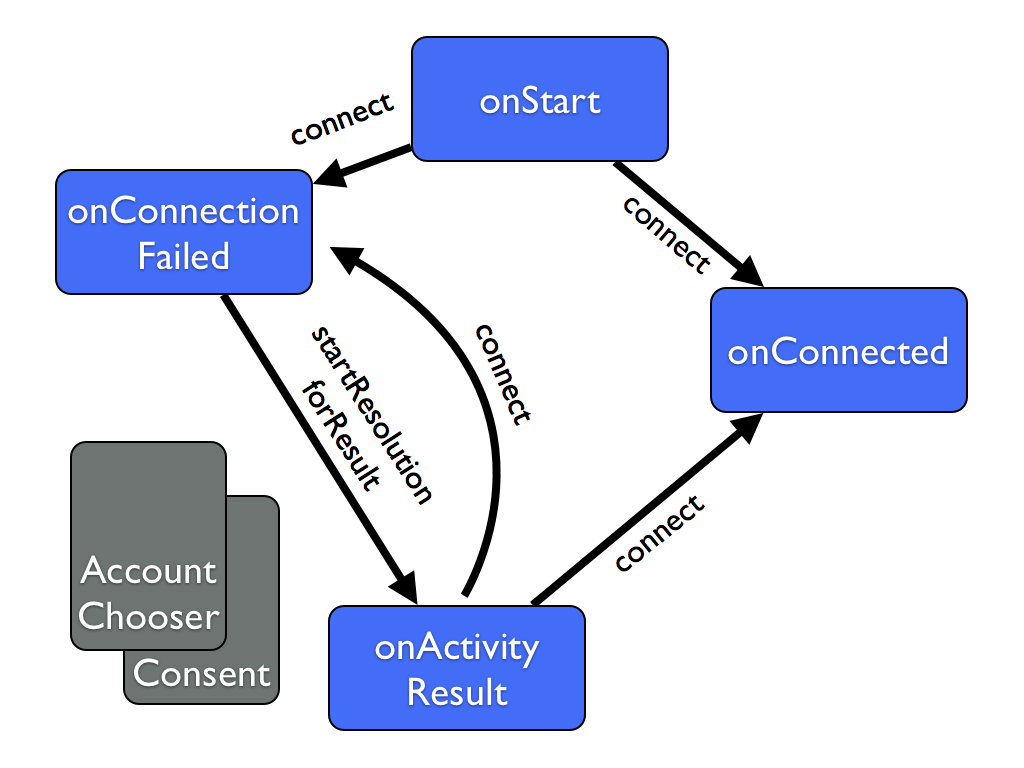
\includegraphics[width=0.8\linewidth]{img/googleclientflow.png}
\caption{Google Client basic life cycle\cite{googleapiclient-lifecycle}}
\label{fig:googleclientlifecycle}
\end{figure}
The blue boxes represents methods in the activity, and the two grey boxes represents other activities. The method \textit{onStart()} is called upon the activity start up, and we immediately try to sign in. This can either succeed or fail, if it fails \textit{onConnectionFailed} will be called, this will happen if the user has not yet consented with the Google+ sign in, the system now awaits for the user to press the sign in button. 
When the user presses the sign in button, the application opens an account chooser activity, only if the user has multiple Google accounts. 
After selecting the account that the user want to use a consent activity will show, presenting the user with permissions that the application should be allowed to access. When the user has granted the application access, the result of the consent activity is returned to \textit{onActivityResult()} and if the user has granted the application access, the user is signed in.
